\documentclass[12pt]{article}

\usepackage{fullpage}
\usepackage{graphicx, rotating, booktabs} 
\usepackage{times}
\usepackage{fbb} 
\usepackage{natbib} 
\usepackage{indentfirst} 
\usepackage{setspace}
\usepackage{grffile} 
\usepackage{hyperref}
\usepackage{adjustbox}
\usepackage{multirow} 
\usepackage{amsmath}
\usepackage[labelfont={bf},textfont=it,labelsep=period]{caption}
\setcitestyle{aysep{}}
\usepackage{sectsty}
% for the big table
\usepackage{afterpage}
\usepackage{array}
\usepackage{lscape}
\usepackage{longtable}
\usepackage{float}
\sectionfont{\Large}
\subsectionfont{\noindent\large\textit}
\subsubsectionfont{\normalsize}


\singlespace
\title{\textbf{Appendix: Using Hierarchical Models to Estimate Heterogeneous Effects}}

\date{}
\bibliographystyle{apsr}

\begin{document}


\maketitle 

\singlespace 

\tableofcontents


\section{Tomz and Weeks Reanalysis}

This summarizes a heterogeneous treatments model of \citep{TomzWeeks2021} and details the underlying \textsf{R} code. 

\subsection{Heterogeneous Treatments} 

Here, I examine how the impact of alliances varies with other factors in the experiment, especially costs, stakes, region and partner democracy.
The heterogeneous treatment model corroborates TW's conclusion that alliances exert the greatest impact in instances when public opinion is otherwise skeptical of intervention.

\autoref{fig:tw-het-treat} supports TW's findings that alliances exert the most influence in situations where the public is otherwise unlikely to intervene. 
This figure shows the impact of alliances in unique combinations of all other experimental treatments. 
For a hypothetical democracy in Eastern Europe where intervention has high stakes, alliances exert minimal impact on public attitudes. 
In low-stakes and high cost interventions to support African, Asian or Latin American dictators, alliances increase support for intervention by 50\%. 
Beyond these systematic differences, random variation that is not attributed to the other treatments is roughly 6\%. 


\begin{figure}[htpb]
	\centering
		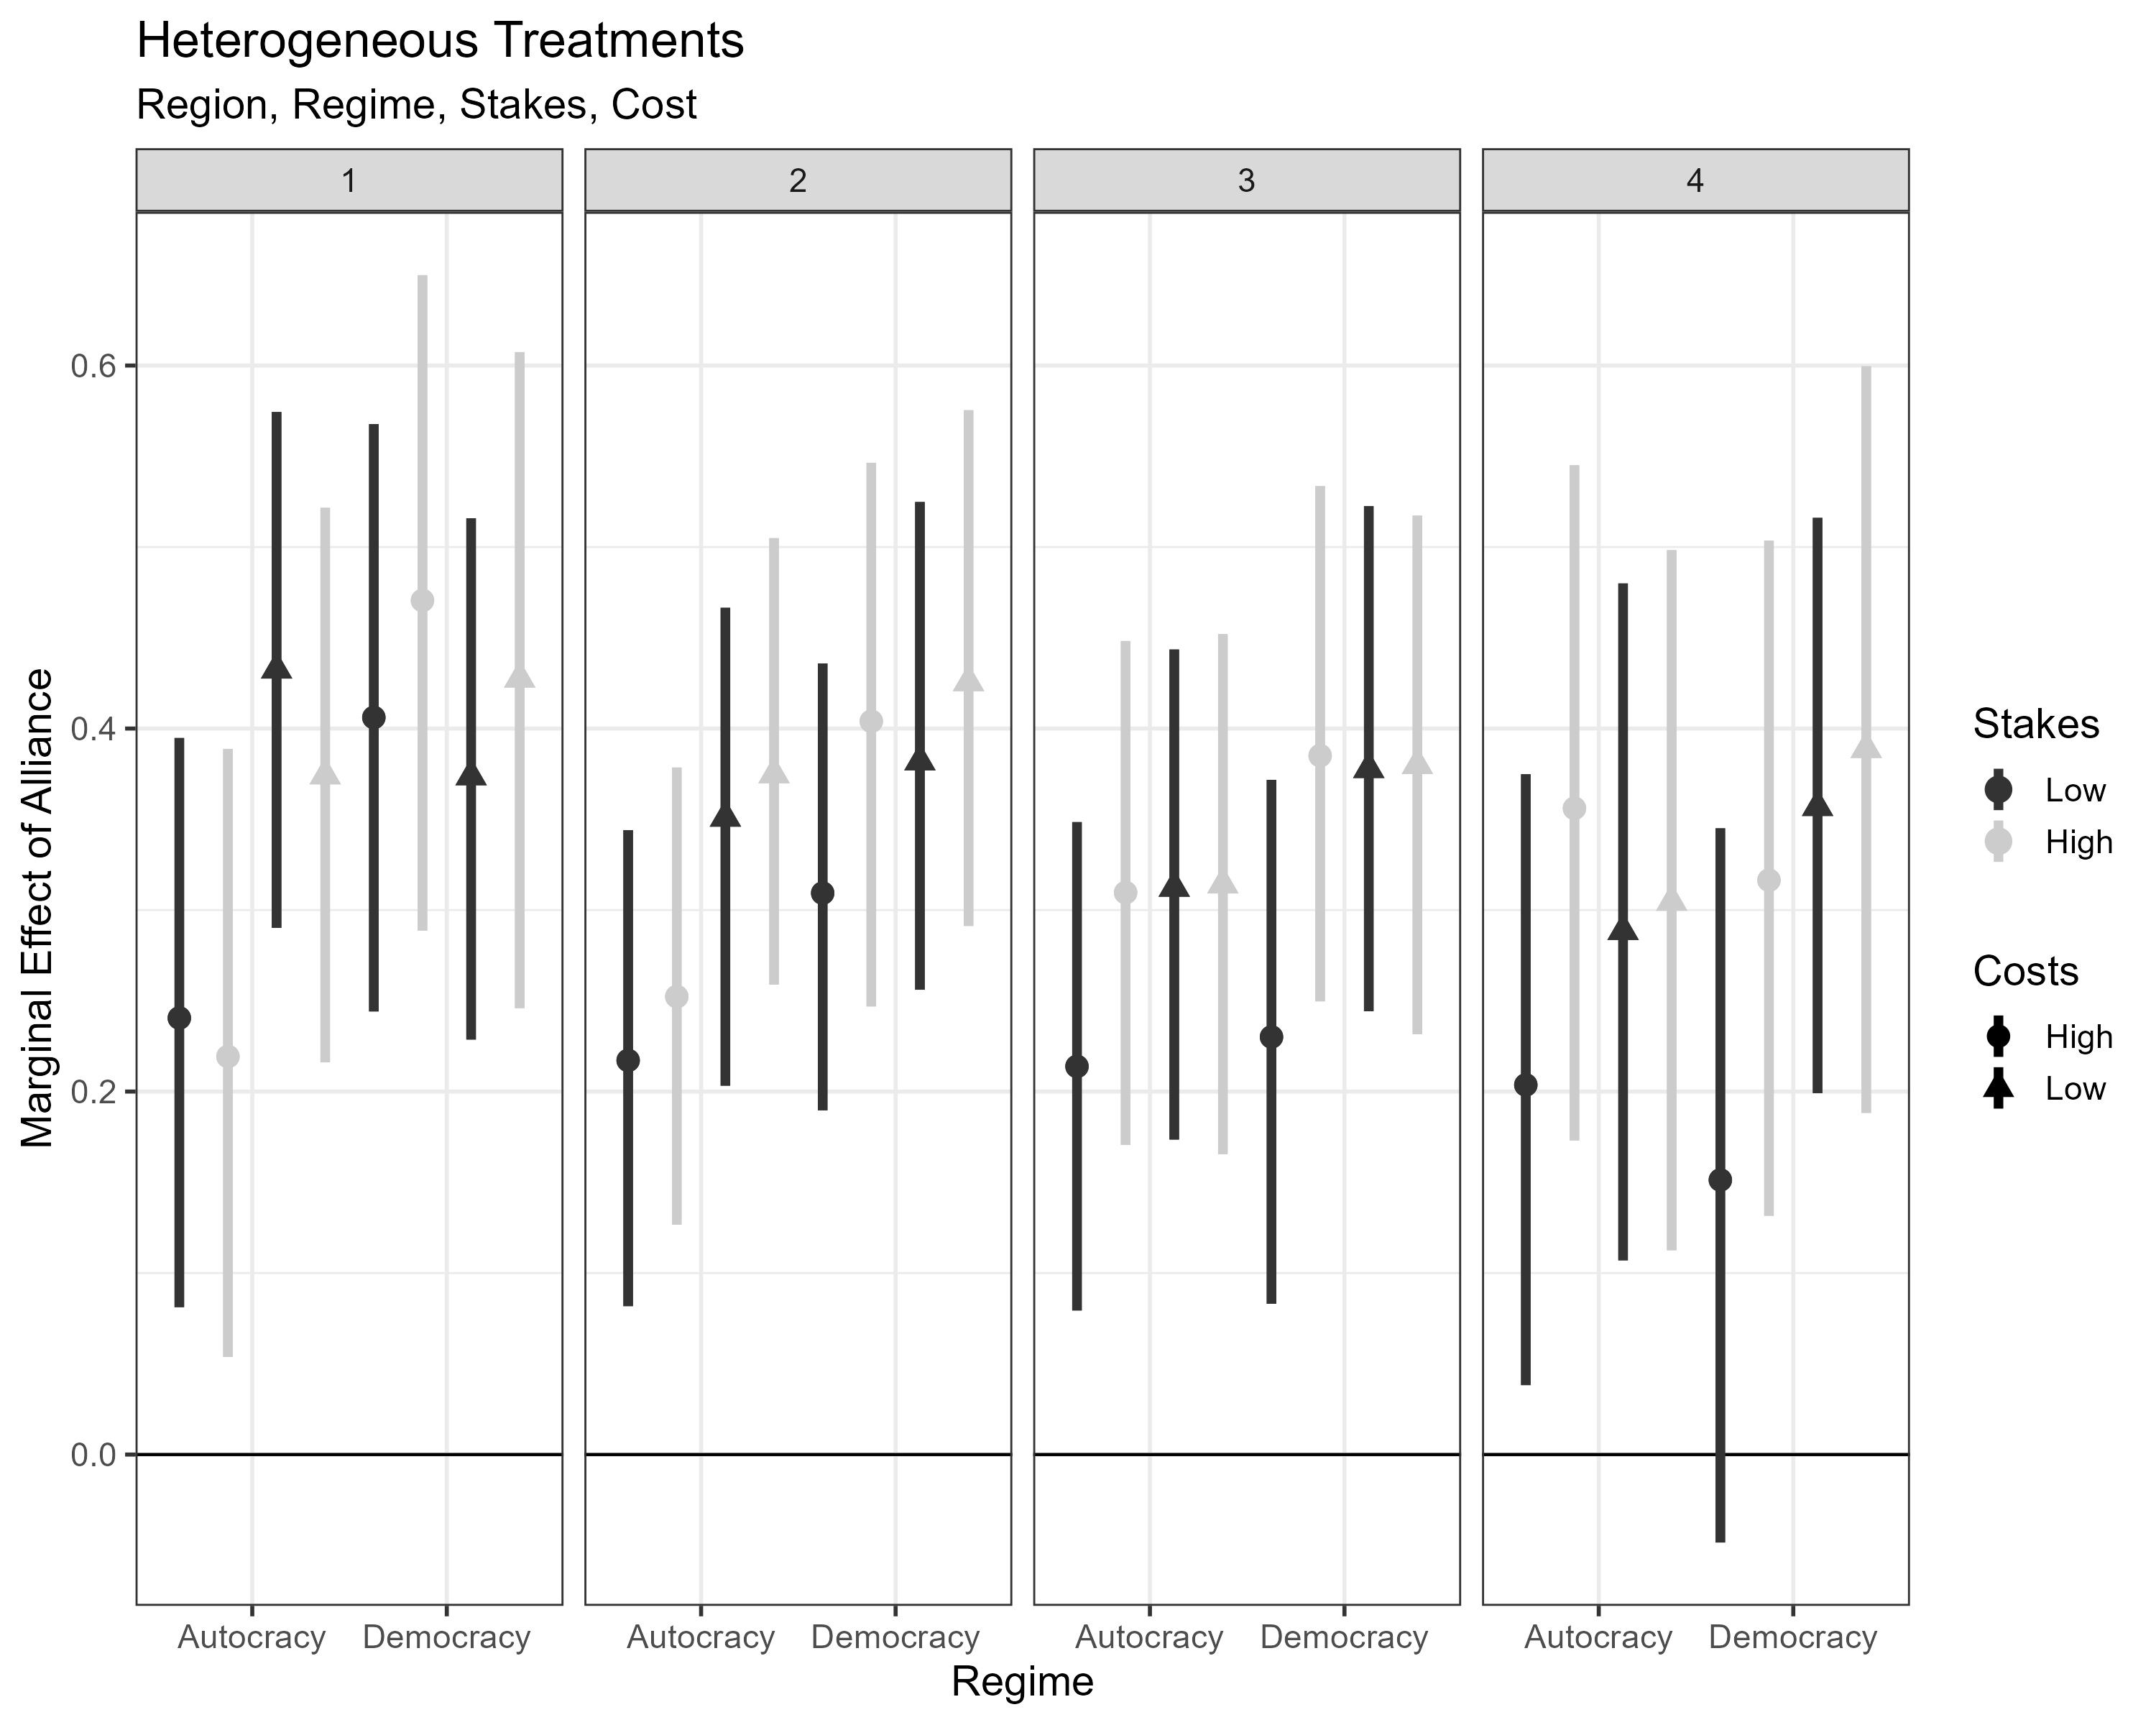
\includegraphics[width=0.95\textwidth]{tw-het-treat.png}
	\caption{Estimated impact of military alliances on public support for war across hypothetical region, costs, stakes and partner regime. Colors distinguish stakes, point shapes mark different costs, and estimates are grouped by regime type. Point estimates give the posterior median and error bars summarize the 95\% credible interval.}
	\label{fig:tw-het-treat}
\end{figure}


\subsection{R Code: Tomz and Weeks Reanalysis}

First, the following model formula expresses a heterogeneous treatments model where the impact of alliances varies with the regime under attack, the stakes, the costs, and the region. 
The \verb+treat.group+ indicator marks unique combinations of the regime, stakes, costs and region variables. 
It can also be written as \verb+regime:stakes:costs:region.txt+. 
I also control for gender, race, and three foreign policy dispositions. 

\begin{verbatim}
bf(force ~ 1 + white + male + hawk + intl + 
             alliance*(regime + stakes + costs + region.txt) + 
             (1 + alliance | treat.group) 
\end{verbatim}


The second formula expresses a treatment heterogeneity model where the impact of alliances varies with gender, race, and three foreign policy dispositions. 
The \verb+het.group+ indicator marks unique combinations of the demographic modifiers.
It can also be written as \verb+white:male:intl:hawk+. 
In this model, the other experimental conditions are controls. 

\begin{verbatim}
bf(force ~ 1 + regime + stakes + costs + region.txt +
             alliance*(white + male + intl + hawk) +
             (1 + alliance | het.group) 
\end{verbatim}


\subsection{Priors: Tomz and Weeks Reanalysis}


\autoref{tab:priors} summarizes the prior distributions. 
All priors are weakly informative relative to the scale of the data. 

\begin{table} % Create a table of priors.
\begin{center}
\begin{tabular}{c} 
$ p(\alpha) \sim N(0, 1)$  \\
$ p(\sigma) \sim \mbox{half-}N(0, 1) $ \\
$ p(\sigma_\theta) \sim \mbox{half-}N(0, 1) $ \\ 
$ p(\beta) \sim N(0, .5) $ 
\end{tabular} 
\caption{Summary of Priors in treatment heterogeneity model.} 
\label{tab:priors}
\end{center} 
\end{table} 



\section{Bush and Prather Reanalysis}


In the following, I again demonstrate how the model works by reanalyzing a study by \citet{BushPrather2020} (BP hereafter). 
This study examines how foreign meddling in elections impacts support for economic engagement with the meddler. 
One of their experiments examines how Russian or German engagement in the 2016 US election impacts mass support for trade and investment with those countries.
I use a heterogeneous effects model to check their results and further explore their findings. 


% describe design
BP employ a 2x2x2 factorial experiment.
This design randomizes whether a foreign country is interfering in the 2016 election, the country and their attitude towards Trump and whether the potential economic ties entail greater trade or investment in the United States.
In one meddling treatment, Russia expresses support for Trump and in the other, Germany expresses opposition to Trump. 


BP hypothesize that individuals will prefer economic engagement with states that support their candidate. 
They thus examine how the impact of side-taking varies with the direction of the endorsement, individual political preferences, and the economic issue. 
To do this, they use four tables and figures, and rely on eight t-tests of differences in means between groups of roughly 25 respondents. 


The heterogeneous effects model encapsulates the argument and all tests by estimating the impact of side-taking on economic engagement as a function of which country is involved, a dummy indicator of intention to vote for Clinton, and their interaction. 
The interaction captures the hypothesis that Clinton voters will support engagement with Germany because Germany opposed Trump, and should be positive. 
I also add an indicator of whether the experiment deals with trade or investment. 
The heterogeneous effects equation also includes indicators of female gender and political engagement. 
The political engagement measure is a sum of political knowledge and interest. 


The outcome variable is a scale from one to four that measures support for greater economic engagement with the potential partner. 
To approximate BP's analyses, I use a normal outcome likelihood. 
Because this experimental randomization produced a roughly balanced sample, I do not include any control variables in the outcome equation. 


\begin{figure}[htpb]
	\centering
		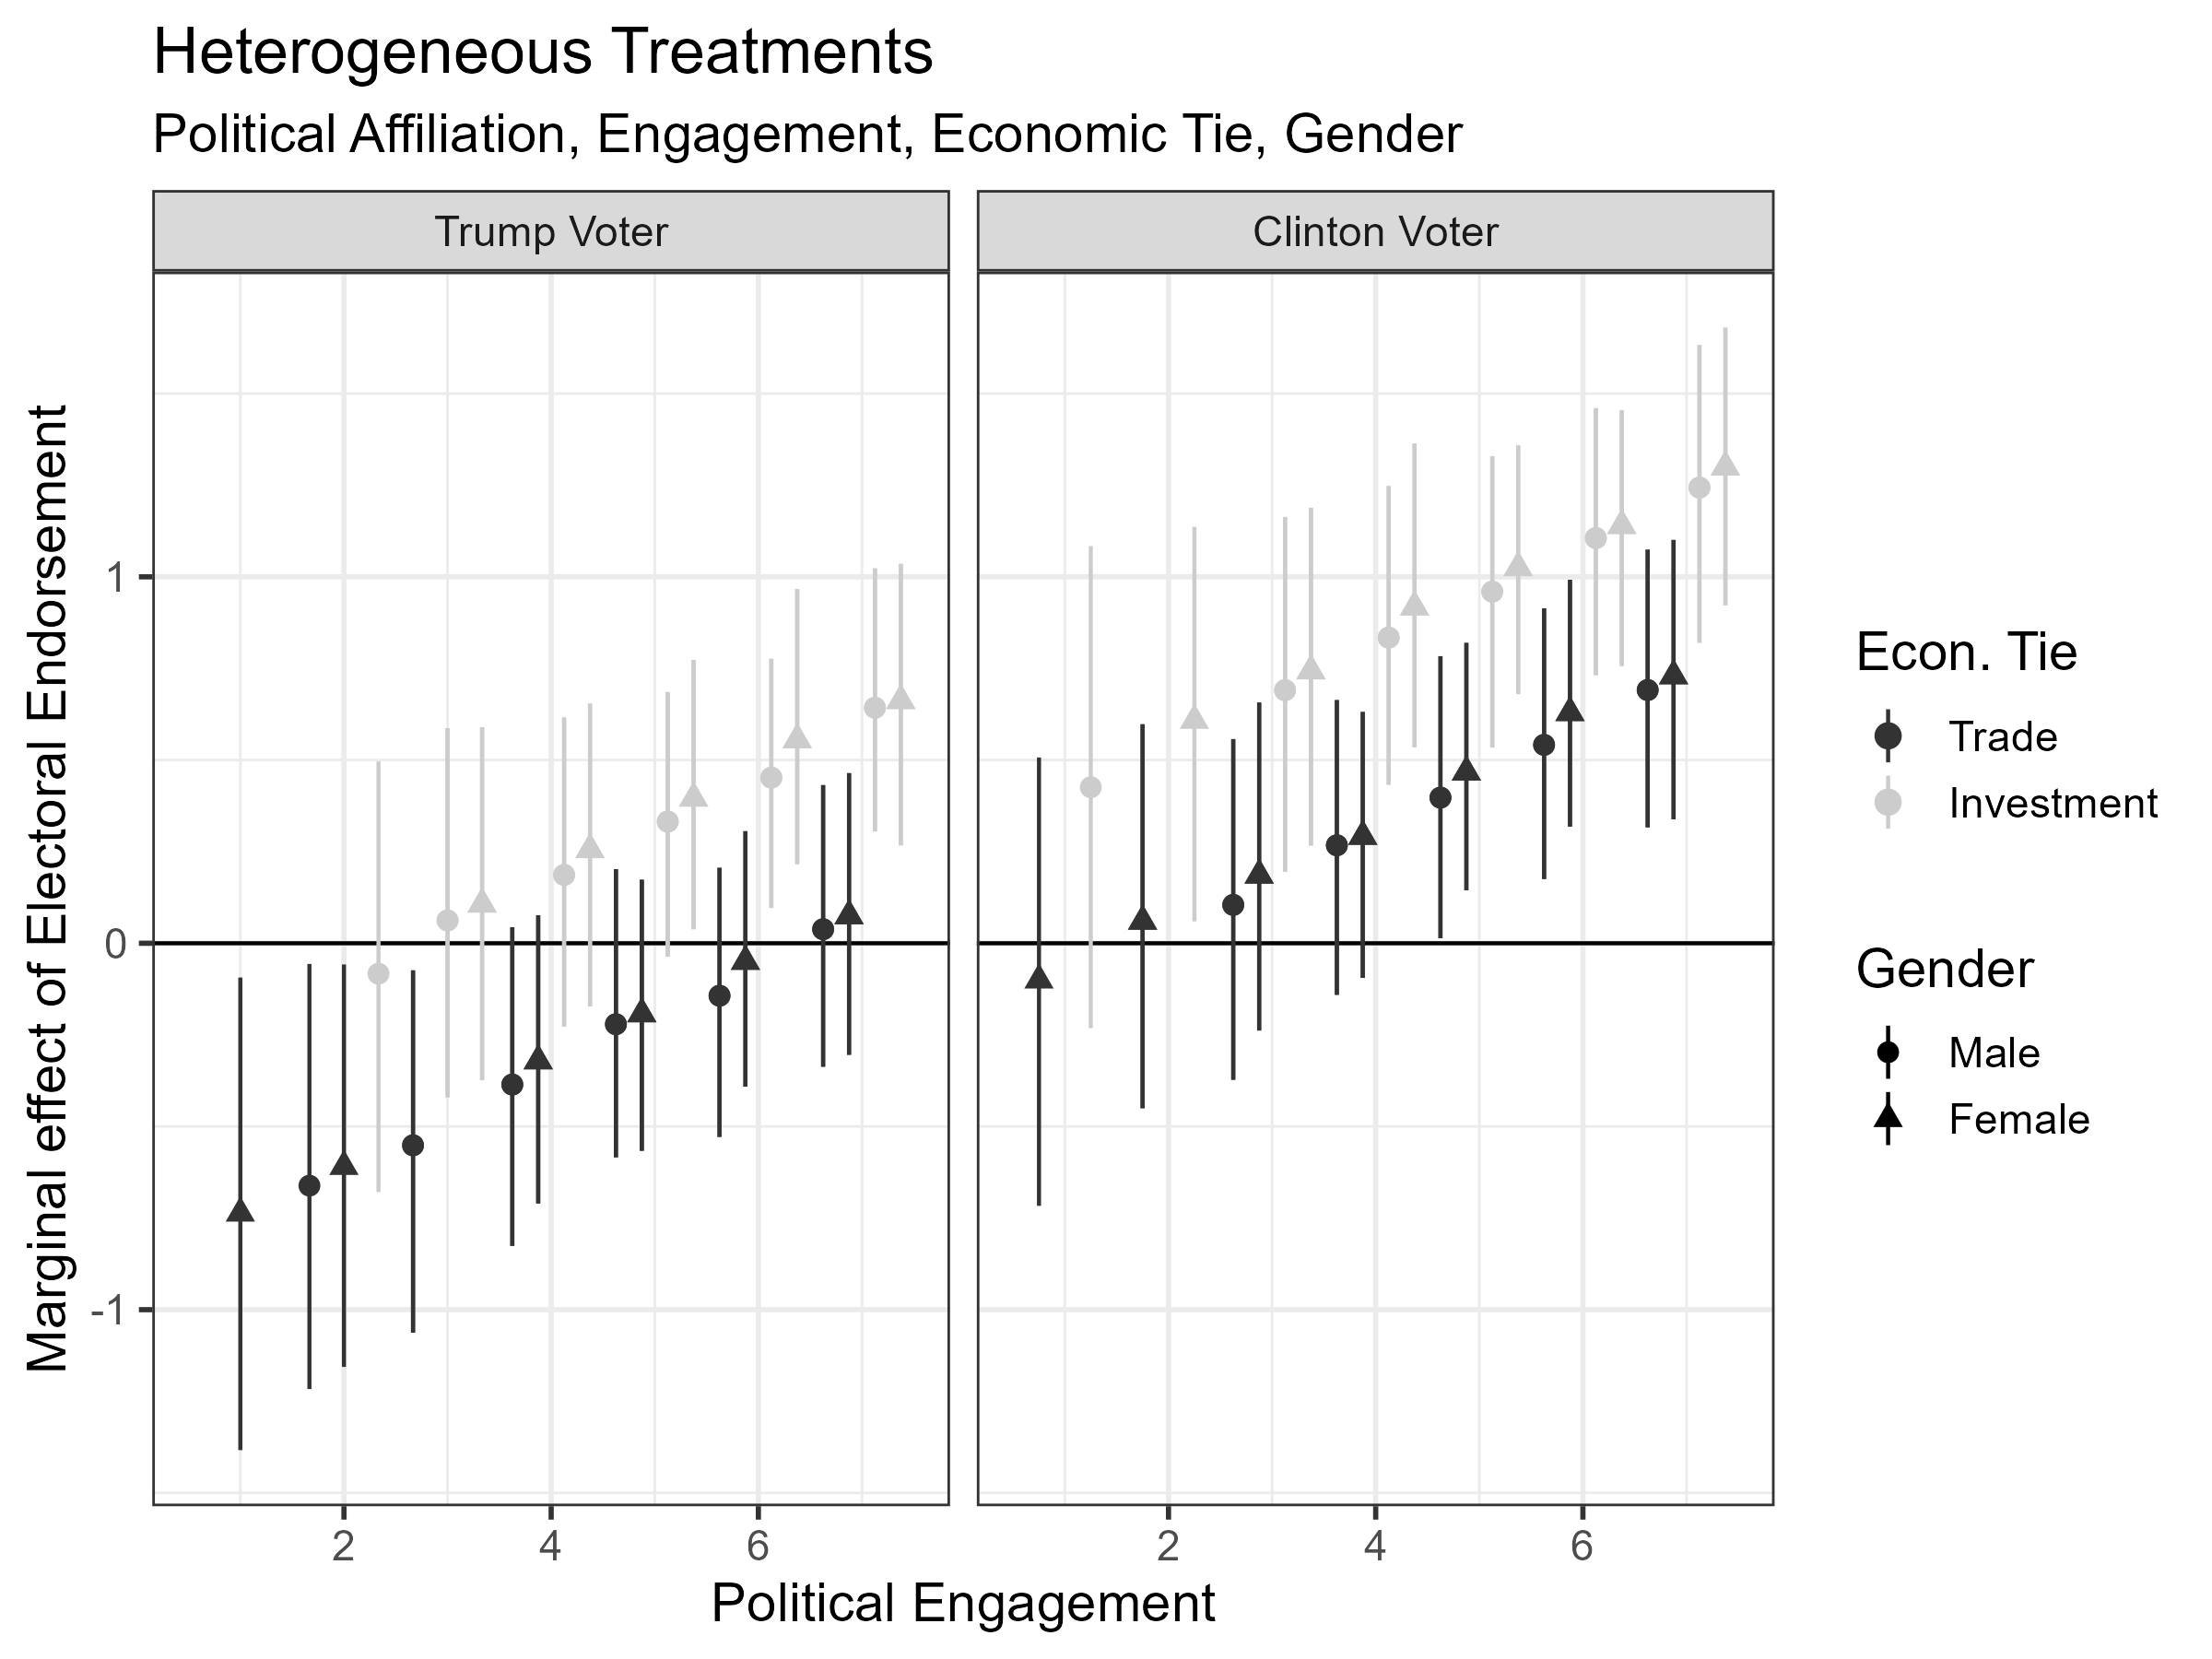
\includegraphics[width=0.95\textwidth]{bp-het-est.png}
	\caption{Heterogeneous effects of German side-taking in US elections on support for economic engagement with Germany. Each estimate reflects a treated group with a unique combination of other treatments and demographic characteristics.}
	\label{fig:bp-het-est}
\end{figure}


These estimates corroborate BP's findings, and also suggest that side-taking exerts the greatest influence on individuals who are highly engaged in politics. 
Clinton voters are more likely to support economic engagement with Germany when Germany has opposed Donald Trump. 
Conversely, some Trump voters oppose greater trade with Germany after the same side-taking. 
The impact of side-taking is also stronger for foreign investment than trade. 
Individuals are more willing to support investment than trade.


Side-taking exerts the most influence on individuals who are highly engaged in politics. 
Engaged Clinton voters respond most to German side-taking against Trump. 
Among these respondents, side-taking increases support for economic engagement by .5 or more, which is a large effect on an outcome that ranges from one to four. 


\singlespace
 
\bibliography{../../MasterBibliography} 


\end{document}